\section{The setting}

\begin{frame}\frametitle{\secname}
    
\underline{Data:}

observations: $\big\{ \vec{x}^{(\alpha)} \big\}, \alpha = 1, \ldots, p; \quad \vec{x} \in \R^N$

$$
\vec x = \rmat{
x_1\\
x_2\\
\vdots\;\,\\
x_N
}
$$

Our entire dataset:
\[
\vec X = 
\left(
\begin{array}{cccc}
\Big| & \Big| & &\Big| \\[3mm]
\vec x^{(1)} & \vec x^{(2)} & \cdots &\vec x^{(p)}\\[2mm]
\Big| & \Big| & &\Big|
\end{array}
\right) \in \R^{N \times p}
\]

\end{frame}

\section{Dimensionality Reduction}

\begin{frame}\frametitle{\secname}
We want to reduce the number of elements in $\vec x \in \R^N$
while retaining as most of the intrinsic information content.

\question{For what purpose?}

\question{What is the difference between dimensionality reduction and compression, if any?}

\end{frame}

%\newpage
\subsection{Simple truncation}




\begin{frame}\frametitle{\subsecname}

\begin{center}
\begin{minipage}{0.3\textwidth}

	%\begin{table}[]
	%\centering
	\resizebox{\textwidth}{!}{%
	\begin{tabular}{c|cccc}
			  & \multicolumn{1}{c}{$\vec x^{(1)}$} & \multicolumn{1}{c}{$\vec x^{(2)}$} & \multicolumn{1}{c}{\ldots} & $\vec x^{(p)}$ \\ \hline%\cline{1-3} \cline{5-5} 
	$x_1$     & -0.2                           & 0.1                            &                       & 0.2       \\ \cline{1-1}
	$x_2$     & 0.1                            & 3.1                            &                       & -1.0      \\ \cline{1-1}
	$x_3$     & 2.5                            & 7.2                            &                       & -0.8      \\ %\cline{1-1}
	  \vdots        &            \vdots                    &     \vdots                          & \begin{tabular}[c]{@{}c@{}}\ldots\vspace{2.5mm}\end{tabular} &      \vdots     \\ %\cline{1-1}
	$x_{N-2}$ & -7.1                           & -3.5                           &                       & 7.0       \\ \cline{1-1}
	$x_{N-1}$ & -10.3                          & -0.3                           &                       & 4.5       \\ \cline{1-1}
	$x_N$     & 4.0                            & 1.3                            &                       & 6.6       \\ \hline
	\end{tabular}%
	}
	%\end{table}
\end{minipage}
\begin{minipage}{0.33\textwidth}
	\begin{center}
		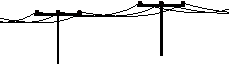
\includegraphics[width=0.99\textwidth]{img/telephone_masts_depth}%
	\end{center}
\end{minipage}
\begin{minipage}{0.3\textwidth}

	\resizebox{\textwidth}{!}{%
	\begin{tabular}{c|cccc}
			  & \multicolumn{1}{c}{$\vec x^{(1)}$} & \multicolumn{1}{c}{$\vec x^{(2)}$} & \multicolumn{1}{c}{\ldots} & $\vec x^{(p)}$ \\ \hline%\cline{1-3} \cline{5-5} 
	$x_1$     & -0.2                           & 0.1                            &                       & 0.2       \\ \cline{1-1}
	$x_2$     & 0.1                            & 3.1                            &                       & -1.0      \\ \cline{1-1}
	$x_3$     & 2.5                            & 7.2                            &                       & -0.8      \\ %\cline{1-1}
	  \vdots        &            \vdots                    &     \vdots                          & \begin{tabular}[c]{@{}c@{}}\ldots\vspace{2.5mm}\end{tabular} &      \vdots     \\ %\cline{1-1}
	$x_{N-2}$ & -7.1                           & -3.5                           &                       & 7.0       \\ \cline{1-1}
	\only<1>{
	$x_{N-1}$ & -10.3                          & -0.3                           &                       & 4.5       \\ \cline{1-1}
	$x_N$     & 4.0                            & 1.3                            &                       & 6.6       \\ \hline
	}
	\only<2>{
	%\hline{\vspace{\dimexpr 2.2ex-\doublerulesep}}
	$\hcancel[red]{x_{N-1}}$ &          \textcolor{red}{?}             &          \textcolor{red}{?}             &                    &    \textcolor{red}{?}   \\ \cline{1-1}
	$\hcancel[red]{x_{N}}$     &                      \textcolor{red}{?}        &               \textcolor{red}{?}            &                   & \textcolor{red}{?}      \\ \hline
	}
	\only<3>{
	%\hline{\vspace{\dimexpr 2.2ex-\doublerulesep}}
	$\color{blue}{x_{N-1}}$ &          \textcolor{blue}{0}             &          \textcolor{blue}{0}          &                    &   \textcolor{blue}{0}  \\ \cline{1-1}
	$\color{blue}{x_{N}}$     &                      \textcolor{blue}{0}        &              \textcolor{blue}{0}           &                   & \textcolor{blue}{0}   \\ \hline
	}
	\end{tabular}%
	}
\end{minipage}

\only<3>{
\vspace{5mm}
	restore $N$-dimensional vector using \textcolor{blue}{simple trunction}.
	
\svspace{5mm}

\begin{minipage}{.8\textwidth}
\begin{minipage}{0.33\textwidth}
	\begin{center}
		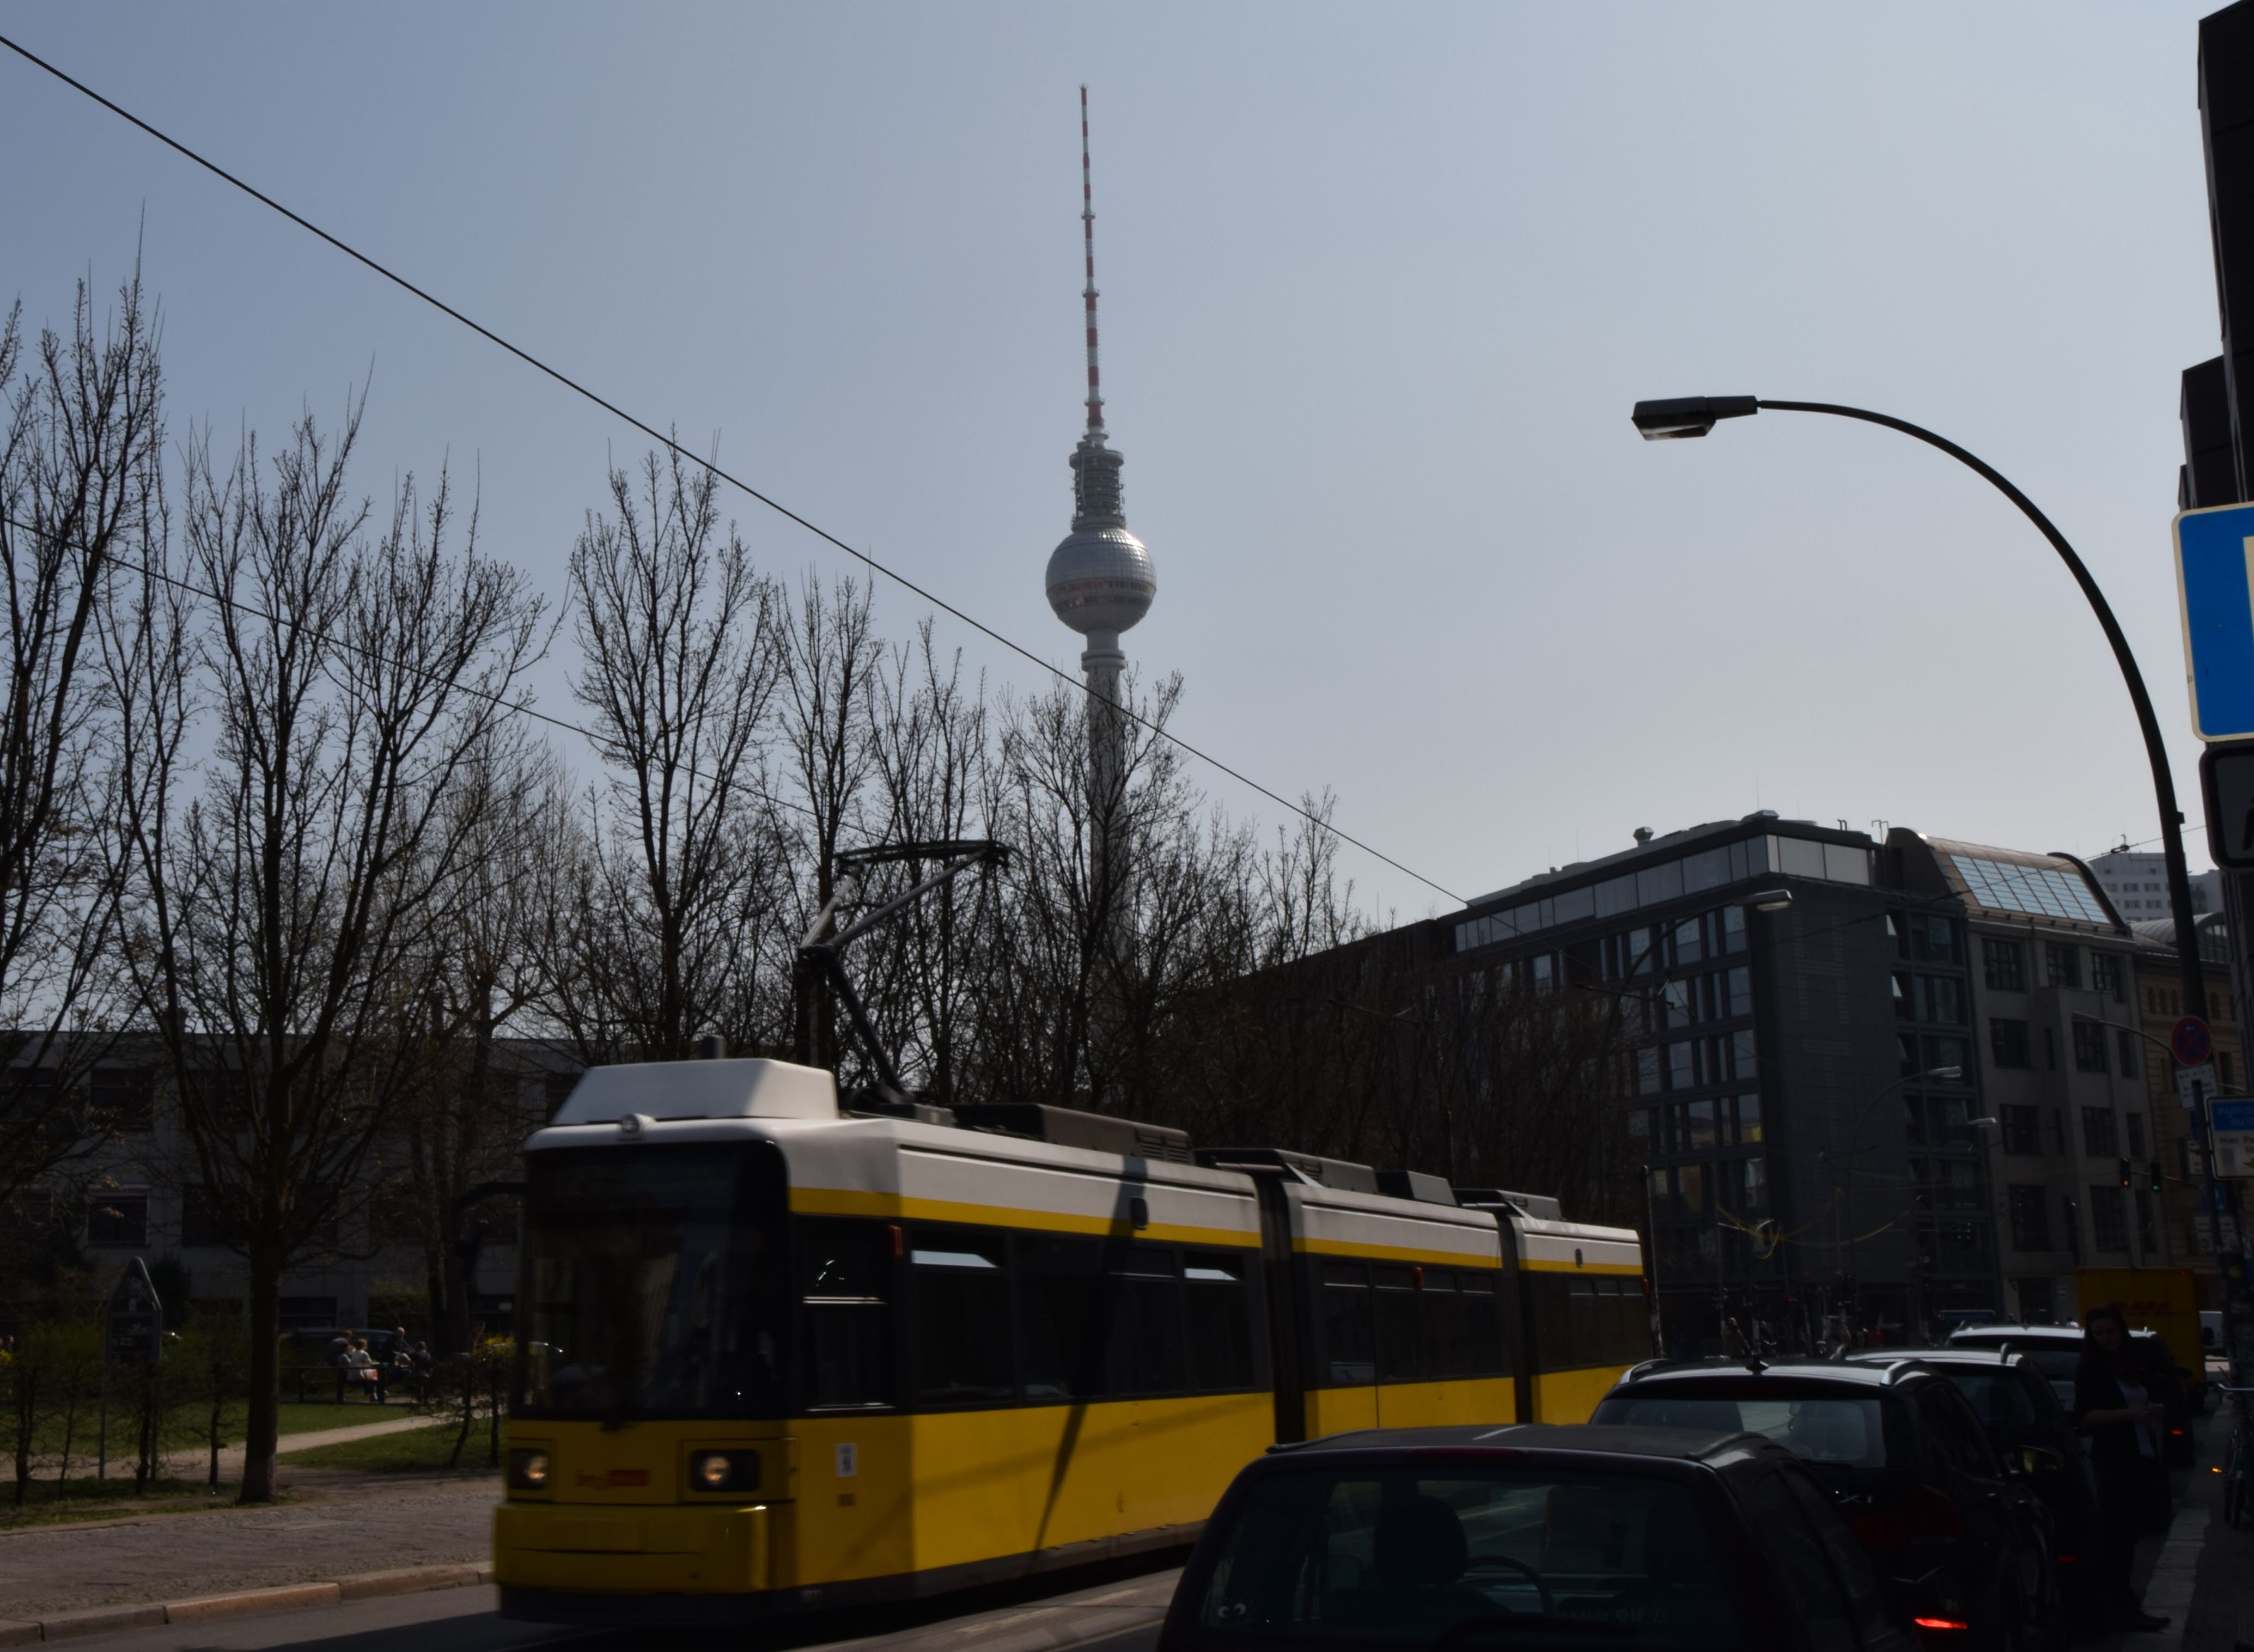
\includegraphics[width=0.99\textwidth]{img/tram}%
	\end{center}
\end{minipage}
\hfill
\begin{minipage}{0.33\textwidth}
	\begin{center}
		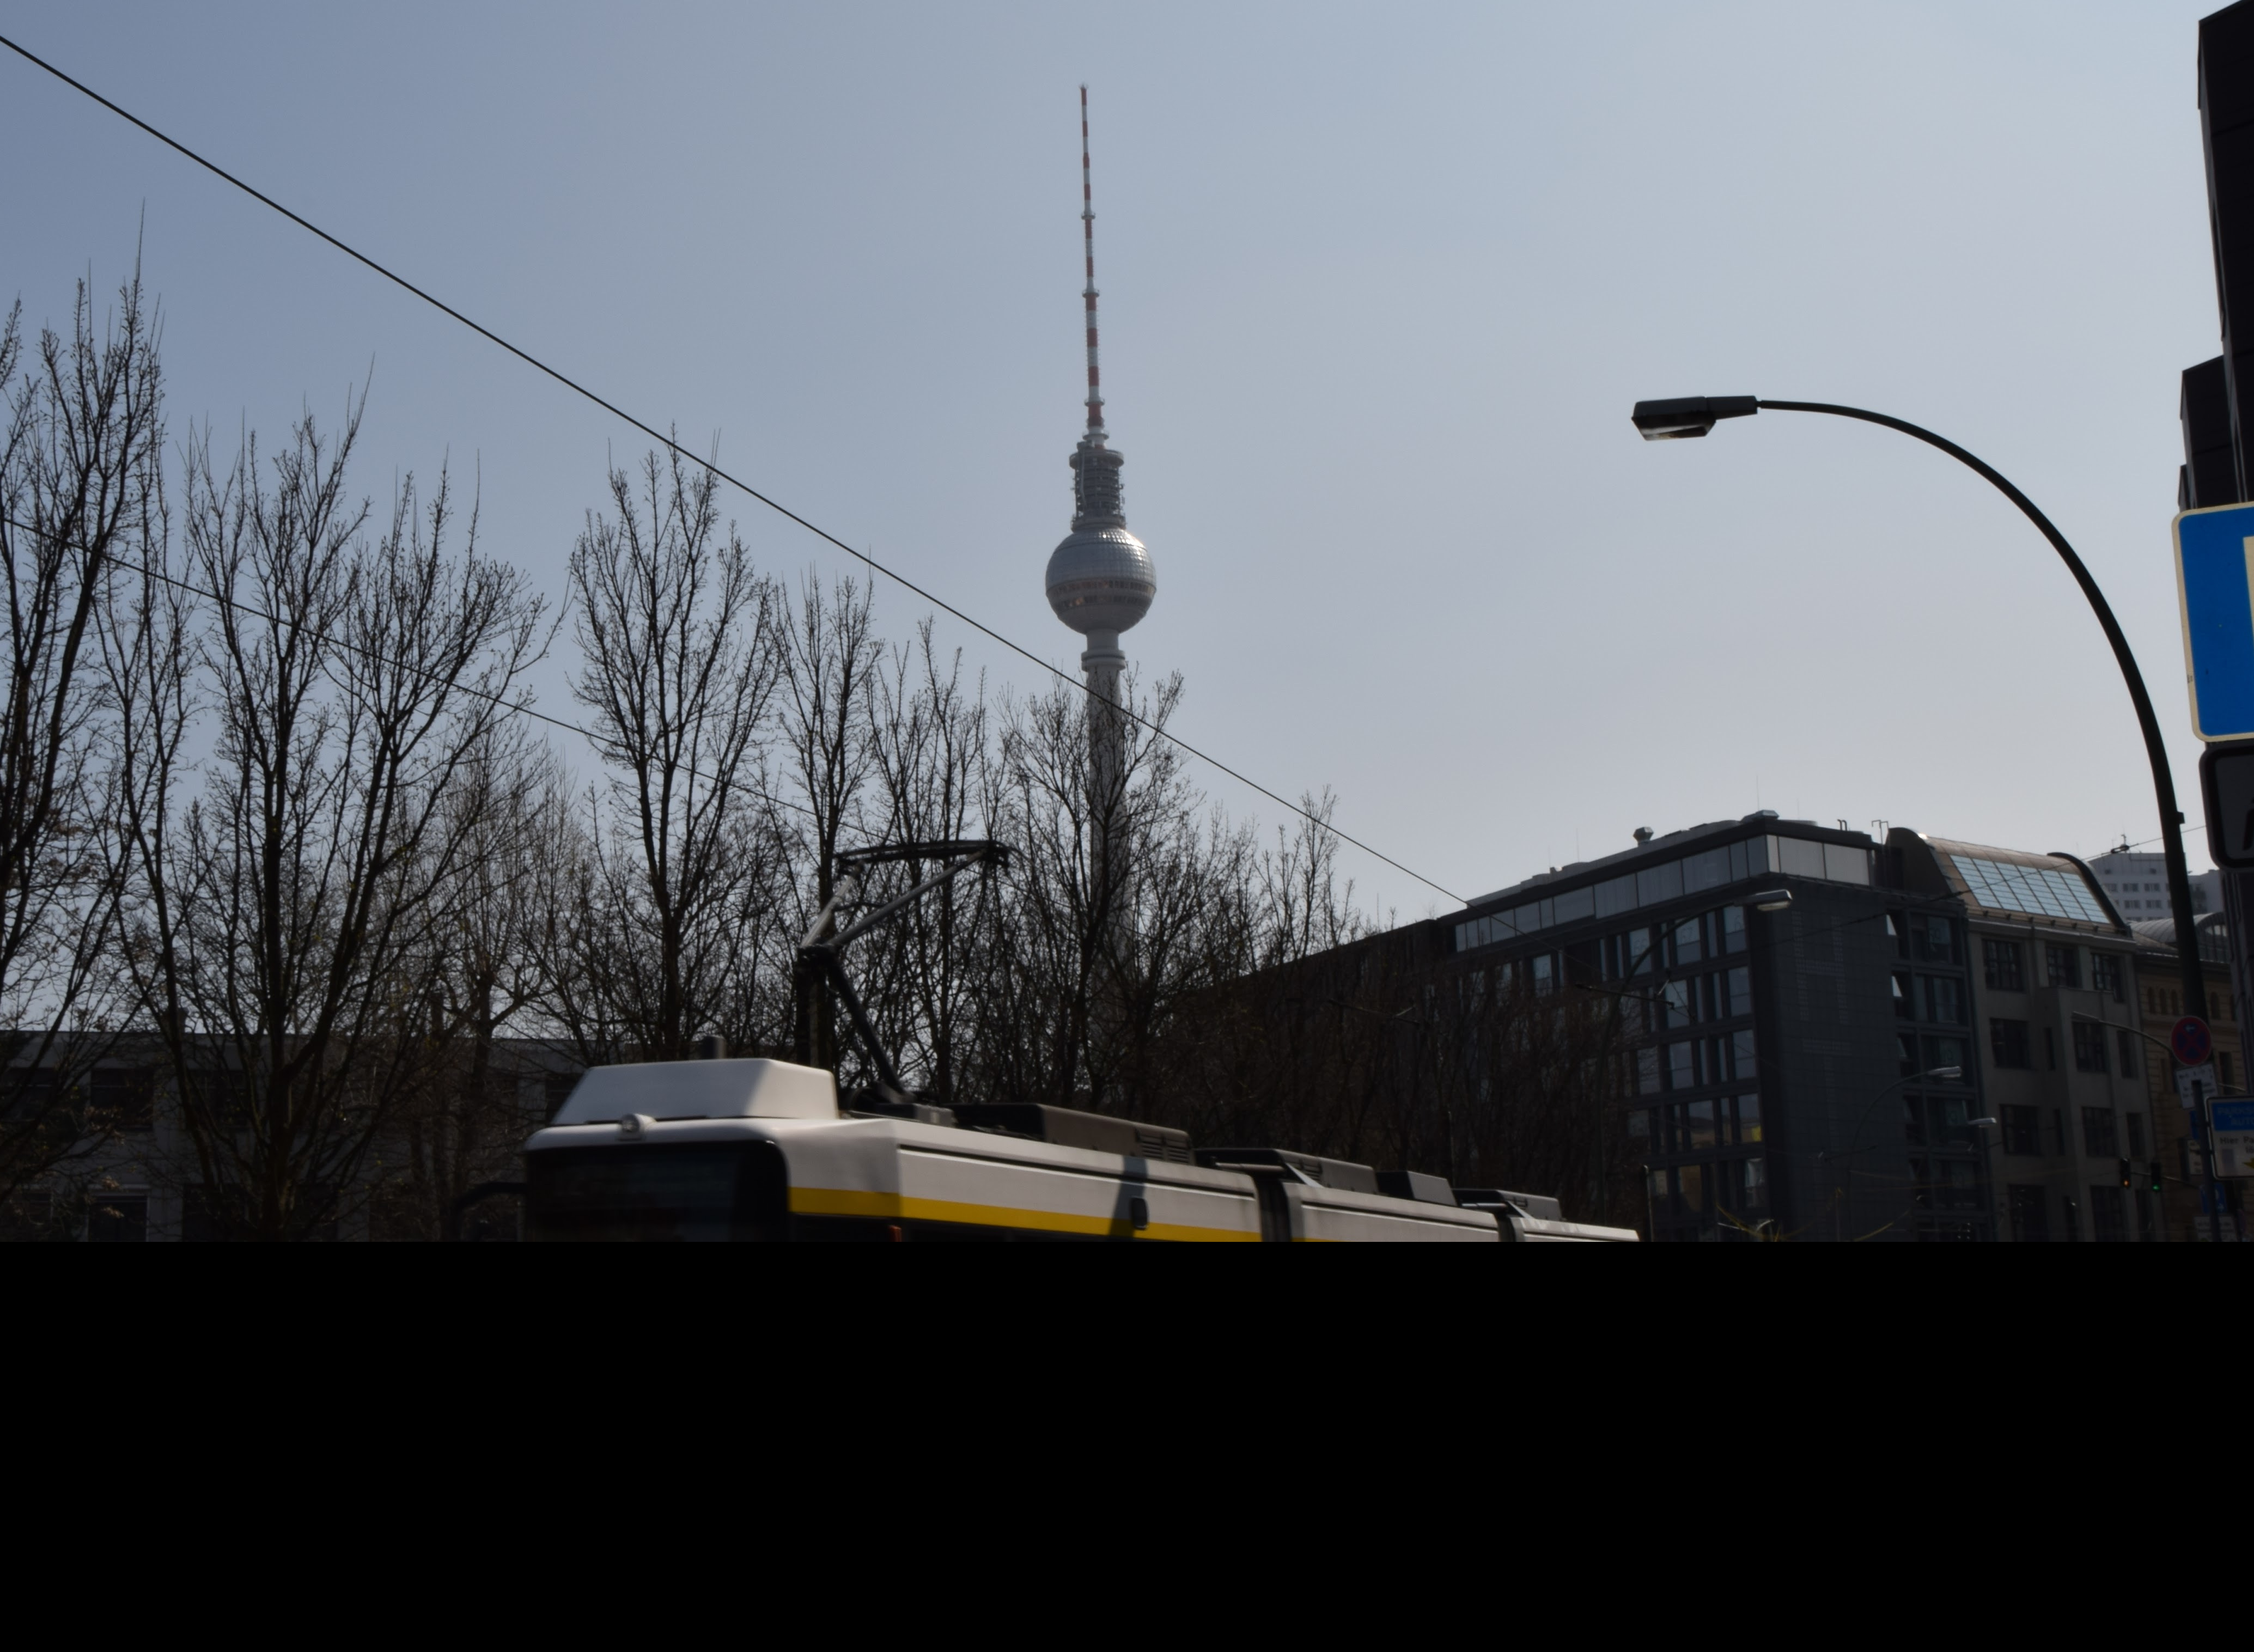
\includegraphics[width=0.99\textwidth]{img/tram_missing}%
	\end{center}
\end{minipage}
\end{minipage}
}



\end{center}

\end{frame}

\subsubsection{Procedure}

\begin{frame}\frametitle{\subsecname:~\subsubsecname}

Let
\slidesonly{\vspace{-5mm}}
\begin{itemize}
\item[]$\vec x \in \R^N$,\\
\item[] w.l.o.g. $\E[\vec x] \eqexcl \vec 0$ (i.e. for each variable $x_i$ its mean $m_i = \sum_{\alpha=1}^{p} x_i^{(\alpha)} \eqexcl 0$)
\end{itemize}

\pause

\begin{enumerate}
\item \underline{Dimensionality Reduction}: From $N$ to $M$: $1 < M\, < N$\\
$\Rightarrow$ simply transmit the first $M$ elements of $\vec x$. 
\pause
\item \underline{Reconstruction}: The recipient reconstructs all $N$ elements by adding zero entries for all missing elements (i.e. \textit{zero-padding}):\\
Let $\widetilde{\vec{x}}$ be the reconstructed observation, where\\ 
 
 \begin{equation}
 % = $ for $j=1,\ldots,M% (perfect reconstruction for the first $M$ elements),
 \widetilde{x}_j = \begin{cases} 
      {x}_j & \text{for}~j=1,\ldots,M \qquad \text{(perfect reconstruction)} \\
      0 & \text{for}~j=M+1,\ldots,N \quad \text{zero-padding} 
   \end{cases}
 \end{equation}
\end{enumerate}

\question{How much error will the recipient accumulate in the case of simple truncation?}

\end{frame}

\subsubsection{Measuring the error}

\begin{frame}\frametitle{\subsecname:~\subsubsecname}

\notesonly{
We measure the MSE between every original point $\vec x$ and its reconstruction $\widetilde{\vec{x}}$.

Let $\widetilde{\vec{x}}$ be the reconstructed observation. }

\slidesonly{\vspace{-7mm}}

\begin{align}
\label{eq:mse}
\visible<1->{
\mathit{MSE}  &=  \frac{1}{p} \sum\limits_{\alpha = 1}^p ( \vec{x}^{(\alpha)} - \widetilde{\vec{x}}^{(\alpha)} )^2
	\notesonly{\\&}=  \frac{1}{p} \sum\limits_{\alpha = 1}^p \sum\limits_{j = 1}^M ( {x}_j^{(\alpha)} - \widetilde{{x}}^{(\alpha)}_j )^2\\
	\intertext{The \textcolor{blue}{first $M$} elements were transmitted perfectly, \textcolor{red}{zero padding} is used to extend the vector to its original size of $N$ elements}
}
\visible<2->{
     &=  \frac{1}{p} \sum\limits_{\alpha = 1}^p \bigg(
     \underbrace{
		{\color{blue}\sum\limits_{j = 1}^M} ( x_j^{(\alpha)} - \widetilde{x_j}^{(\alpha)} )^2
		}_{
		\substack{=0 \\\text{ (perfect transmission)}}
		} 
		+ {\color{red}\sum\limits_{j = M+1}^N} ( x_j^{(\alpha)} - 
	\underbrace{
	\vphantom{\sum\limits_{j = 1}^M ( x_j^{(\alpha)} - \widetilde{x_j}^{(\alpha)} )^2}
	\widetilde{x_j}^{(\alpha)}
	}_{\substack{=0\\ \text{padded}}}
	\;)^2 \bigg)\\
     &=  \frac{1}{p} \sum\limits_{\alpha = 1}^p \sum\limits_{j = M+1}^N ( x_j^{(\alpha)} )^2
     \notesonly{\\&}=  \sum\limits_{j = M+1}^N \frac{1}{p} \sum\limits_{\alpha = 1}^p  ( x_j^{(\alpha)} )^2 \\
     &=  \sum\limits_{j = M+1}^N \sigma_j^2
     }
\end{align}

\end{frame}

\begin{frame}

\slidesonly{
\begin{equation}
\mathit{MSE}  =  \frac{1}{p} \sum\limits_{\alpha = 1}^p ( \vec{x}^{(\alpha)} - \widetilde{\vec{x}}^{(\alpha)} )^2 = \sum\limits_{j = M+1}^N \sigma_j^2
\end{equation}
}

In the case of simple trunctation 
the recipient will end up with an MSE equal to $\sum_{j=M+1}^{N} \sigma_j^2$, where $\sigma_j^2$ is the variance of the $x_j$.
\only<1>{
\begin{equation}
\sigma_j^2 = \E\lbrack~(x_j - m_j)^2~\rbrack \stackrel{m_j=0}{=} \E\lbrack~(x_j)^2~\rbrack
\end{equation}
}

\pause

\slidesonly{\vspace{5mm}}

\underline{Objective:} Rotate/Transform the data s.t. truncating the transformed vector $\vec v \in \R^M$ is optimum in the sense of minimal MSE.


\question{Any ideas?}

\pause

- Sort the $N$ component in $\vec x$ from highest to lowest variance. \notesonly{The transformation here would be some permutation of the idenitty matrix that accomplishes the sorting.}\slidesonly{transformation: permutation of identity matrix}

\question{Is this enough?}

- No, we still have to take the \emph{covariances} into consideration.

\end{frame}

